\documentclass{article}
\usepackage[margin=1.25in]{geometry}
\usepackage{amsmath}
\usepackage{amssymb}
\usepackage{enumitem}
\setlist{nosep}
\usepackage{tcolorbox}
\usepackage[per-mode=fraction]{siunitx}
\usepackage{tikz}

\usetikzlibrary { decorations.pathmorphing, decorations.pathreplacing, decorations.shapes,
  angles, quotes}


\title{Heat Equation -- Back to Basics}
\author{SF Wolf}
\date{\today}

\begin{document}
\maketitle

The heat equation, with power generation is the following:
\[
  \frac{\partial u(x_i,t)}{\partial t} = \alpha \nabla^2 u(x_i,t) + \frac{\dot{q}(x_i,t)}{c_p
    \rho}
\]
In this equation we have two functions which depend on space \((x_i)\) and time \((t)\):
\begin{itemize}
  \item \(u(x_i,t)\) Temperature with units \unit{\kelvin}
  \item \(\dot{q}(x_i,t)\) Power generation density with units \unit{\watt\per\meter^3}
\end{itemize}
And the following physical parameters which depend on the material:
\begin{itemize}
  \item \(\alpha\) Thermal diffusivity with units \unit{\meter^2\per\second}
  \item \(c_p\) Specific heat capacity with units \unit{\joule\per\kilo\gram\per\kelvin}
  \item \(\rho\) mass density with units \unit{\kilo\gram\per\meter^3}
\end{itemize}

\section{Boundary conditions}

Additionally, we consider what happens at a boundary. The heat flux (energy per unit area per
unit time) is:
\[
  \Phi = \left. \kappa\frac{\partial u}{\partial n}\right|_{\text{bdry}}
\]
where \(\kappa\) is another material parameter, the \emph{thermal conductivity} with units
\unit{\watt\per\meter\per\kelvin}. This is used in boundaries between materials as well as edge
boundaries.


\subsection{Material boundaries}

Sometimes, there will be two materials that are next to each other. At the boundary surface, we
will find that the temperature is continuous at all points \((X,Y,Z)\) on the boundary.

\[
  u_1(X,Y,Z,t) = u_2(X,Y,Z,t)
\]

And the heat flux is continuous on the boundary:

\[
  \left. \kappa_1 \frac{\partial u_1}{\partial n}\right|_{(X,Y,Z)} = \left. \kappa_2
    \frac{\partial u_2}{\partial n}\right|_{(X,Y,Z)}
\]

where \(u_1\) and \(k_1\) describe the temperature and thermal conductivity of material 1, and
\(u_2\) and \(k_2\) describe the corresponding quantities of the other material.


\subsection{Edge boundaries}

In general, there are 4 types of boundary conditions that are usually considered for an
\textbf{\emph{outer}} boundary of an object:
\begin{enumerate}
  \item Dirichelet
  \item Neumann
  \item Robin
  \item Radiation
\end{enumerate}
This last type is used infrequently for applications on earth, so I will not go into more
detail on that one.


\subsubsection{Dirichelet}

For points \((x_b,y_b,z_b)\) on the outer boundary of an object, the temperature is determined
for us.
\[
  u(x_b,y_b,z_b,t) = f(x_b,y_b,z_b,t)
\]
where \(f\) is a known function of space and/or time.


\subsubsection{Neumann}

This is for a perfectly insulated object. That is, for points \((x_b,y_b,z_b)\) on the outer
boundary of an object, the heat flux must be zero:

\[
  \left. \frac{\partial u(x,y,z,t)}{\partial n}\right|_{(x_b,y_b,z_b)} = 0
\]


\subsubsection{Robin}
This describes convection. That is the heat flux depends on the difference between the
surrounding temperature \(T\) and the temperature on the boundary.
\[
  \left. \kappa \frac{\partial u(x,y,z,t)}{\partial n}\right|_{(x_b,y_b,z_b)} = h (T -
  u(x_b,y_b,z_b,t))
\]
where \(h\) is the \emph{heat transfer coefficient} for a material with units
\unit{\watt\per\meter^2\per\kelvin}.


\begin{tcolorbox}[title=In Summary]
  The heat equation is:
  \[
    \frac{\partial u(x_i,t)}{\partial t} = \alpha \nabla^2 u(x_i,t) + \frac{\dot{q}(x_i,t)}{c_p
      \rho}
  \]
  where
  \begin{itemize}
    \item $u(x_i,t)$ describes the temperature with units of \unit{\kelvin}
    \item $\dot{q}(x_i,t)$ describes the ``internal'' power generation density with units of
    \unit{\watt\per\meter^3}
  \end{itemize}
  The heat flux through a surface is:
  \[
    \kappa \frac{\partial u}{\partial n}
  \]
  where $n$ is the spatial coordinate in the direction of the surface normal. And the heat flux
  from a surface to the environment is described by:
  \[
    h\Delta T
  \]
  where $\Delta T$ is the difference in temperature between the surface and the
  environment. Finally, materials are described using the following properties:
  \begin{center}
    \begin{tabular}{lcc}
      \hline\hline
      Name &Symbol &Unit \\
      \hline
      Thermal diffusivity & $\alpha$ & \unit{\meter^2\per\second} \\
      Specific heat capacity & $c_p$ & \unit{\joule\per\kilo\gram\per\kelvin} \\
      Mass density & $\rho$ &\unit{\kilo\gram\per\meter^3} \\
      Thermal conductivity & $\kappa$ & \unit{\watt\per\meter\per\kelvin} \\
      Heat Transfer coefficient & $h$ & \unit{\watt\per(\meter^2\kelvin)} \\
      \hline\hline
    \end{tabular}
  \end{center}
\end{tcolorbox}

\section{Power Generation}
Often, this can take several forms. Of interest to me are the following:
\begin{itemize}
  \item Power generation due to solar intensity
  \item Power generation due to a heat source/sink at a specific position.
\end{itemize}

\subsection{Solar Intensity}
For light with intensity $I_0$ incident on a surface as depicted below:
\begin{center}
  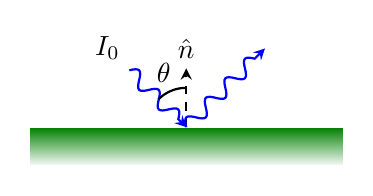
\begin{tikzpicture}[thick,>=stealth]
    \shadedraw [color=white, top color=black!50!green, bottom color=white] (-2,0) rectangle
    (2,-0.5); \node (A) at (-1,1) {$I_0$}; \coordinate (O) at (0,0); \node (B) at (0,1)
    {$\hat{n}$}; \coordinate (C) at (1,1); \draw[decorate, decoration={coil, aspect=0},->,blue]
    (A) -- (O); \draw[dashed, ->] (O) -- (B); \draw pic ["$\theta$",draw,angle
    eccentricity=1.5]{angle=B--O--A}; \draw[decorate, decoration={coil, aspect=0},->,blue] (O)
    -- (C);
  \end{tikzpicture}
\end{center}

The power deposited in the surface is:
\[
  \dot{q} = \frac{I_0 \cos^2\theta}{\delta}
\]
where $\delta$ is the ``penetration depth'' of the light with units \unit{\meter}.


\subsection{Heat source/heat sink}
Oftentimes, what happens in reality is that a blower with extract (or deposit) a volume of air
from (or to) a room, for example through a return or a vent and model this (for point sources)
as follows:
\[
  \dot{q} = \pm \beta\rho c_p u(x,y,z,t) \delta(x-x_s)\delta(y-y_s)\delta(z-z_s)
\]
where the $\delta(x-x_s)$ are the Dirac delta functions and $(x_s,y_s,z_s)$ are coordinates of
the point source/sink and $\beta$ is the blower strength (volume/time or
\unit{\meter^3\per\second}) of the air handler.

\subsection{No Power Generation}
Note, that with no power generation, the ``Temperature Units'' don't matter. It's only when we
are working with power sources/sinks that we need to use SI units.

Let
\[
  u(x,y,z,t) = a f(x,y,z,t) + b
\]
for some $a,b\in\mathbb{R}$. Furthermore let $u(x,y,z,t)$ solve the heat equation with
$\dot{q}(x,y,z,t)=0$. Therefore:
\[
  \frac{\partial u}{\partial t} = \alpha \nabla^2u \rightarrow \frac{\partial}{\partial t}(a
  f(x,y,z,t) + b) = \alpha \nabla^2\left(a f(x,y,z,t) + b\right)
\]
Because of the properties of the derivative, we find
\[
  \frac{\partial f}{\partial t} = \alpha \nabla^2f
\]
So absolute temperature is not required.

\section{Example solutions}

For all of these examples, I'm going to consider a 3D, rectangular prism that goes from
$(0,0,0)$ to $(L,W,H)$.

In general, I'm going to stay in Cartesian coordinates, as such, I'll assume a separable
solution:
$$
u(x,y,z,t) = X(x)Y(y)Z(z)T(t)
$$
We can substitute this into the heat equation to find:
\[
  \frac{\frac{dT}{dt}}{\alpha T} = \frac{\frac{d^2X}{dx}}{X} + \frac{\frac{d^2Y}{dy}}{Y} +
  \frac{\frac{d^2Z}{dz}}{Z}
\]
Since we have \texttt{(function of time) = (function of space)}, both have to be equal to a
constant. By convention, we choose that constant to be $-\lambda$. Let's start by looking at
the right hand side of that equation:
\[
  \frac{\frac{d^2X}{dx}}{X} + \frac{\frac{d^2Y}{dy}}{Y} + \frac{\frac{d^2Z}{dz}}{Z} = -\lambda
\]
We can re-arrange this as follows:
\[
  \frac{\frac{d^2X}{dx}}{X} = -\frac{\frac{d^2Y}{dy}}{Y} - \frac{\frac{d^2Z}{dz}}{Z} -\lambda
\]
Here we have \texttt{(function of x) = (function of y) + (function of z) + constant} and by the
same logic as above, we get that they have to be equal to a constant, let's call this $k_x^2$.

Following that pattern we can rewrite the heat equation as the following four ODEs:
\begin{align*}
  T'(t) + \alpha\lambda T(t) &= 0 \\
  X''(x) + k_x^2 X(x) &= 0 \\
  Y''(y) + k_y^2 Y(y) &= 0 \\
  Z''(z) + k_z^2 Z(z) &= 0 \\
\end{align*}
where $\lambda = k_x^2 + k_y^2 + k_z^2$. And the general solutions can be:

If all $k_{xyz}$ are real and all $k_{xyx} \neq 0$:
\begin{align*}
  T(t) &= \exp\left(-\alpha \lambda t\right) \\
  X(x) &= A_x \sin\left(k_x x\right) + B_x \cos\left(k_x x\right) \\
  Y(y) &= A_y \sin\left(k_y y\right) + B_y \cos\left(k_y y\right) \\
  Z(z) &= A_z \sin\left(k_z z\right) + B_z \cos\left(k_z z\right) \\
  \lambda &= k_x^2 + k_y^2 + k_z^2
\end{align*}

If all $k_{xyx} = 0$ (and $\lambda = 0$):
\begin{align*}
  T(t) &= 1 \\
  X(x) &= A_x x + B_x \\
  Y(y) &= A_y y + B_y \\
  Z(z) &= A_z z + B_z \\
\end{align*}

If all $k_{xyz}$ are imaginary and all $k_{xyx} \neq 0$, and $\lambda < 0$:
\begin{align*}
  T(t) &= \exp\left(-\alpha \lambda t\right) \\
  X(x) &= A_x \sinh\left(k_x x\right) + B_x \cosh\left(k_x x\right) \\
  Y(y) &= A_y \sinh\left(k_y y\right) + B_y \cosh\left(k_y y\right) \\
  Z(z) &= A_z \sinh\left(k_z z\right) + B_z \cosh\left(k_z z\right) \\
  \lambda &= k_x^2 + k_y^2 + k_z^2
\end{align*}




\subsection{Example 1: Dirichelet BC's}
Assume the temperature is 0 everywhere on the boundary

$$
0 = u(0,y,z,t) = u(l,y,z,t) = u(x,0,z,t) = u(x,w,z,t) = u(x,y,0,t) = u(x,y,h,t)
$$

With this in mind, the boundary conditions become:
\[
  0 = X(0) = X(L) = Y(0) = Y(W) = Z(0) = Z(H)
\]

If we apply these conditions, we find:
\begin{itemize}
  \item $\lambda = 0$ is not a meaningful solution because $A_x=A_y=A_z=B_x=B_y=B_z=0$
  \item $\lambda < 0$ is not a meaningful solution because $A_x=A_y=A_z=B_x=B_y=B_z=0$
  \item $\lambda > 0$ is the only possible solution with
\end{itemize}
\[
  B_x = B_y = B_z = 0 \quad k_x=\frac{i\pi}{L} \quad k_y = \frac{j\pi}{W} \quad k_z =
  \frac{k\pi}{H}
\]
where $i,j,k$ are non-zero, positive integers. As a result, we get:
\begin{align*}
  u(x,y,z,t) &= \sum_{klm} a_{klm}\exp\left(-\alpha\lambda_{klm}t\right)
               \cos\left(\frac{k\pi x}{L}\right) \cos\left(\frac{l\pi y}{W}\right)
               \cos\left(\frac{m\pi z}{H}\right) \\
  \lambda_{klm} &= \frac{k^2\pi^2}{L^2} + \frac{l^2\pi^2}{W^2} + \frac{m^2\pi^2}{H^2}
\end{align*}
where $a_{klm}$ are arbitrary constants that depend on the initial condition. Given some
initial condition:
\[
  u(x,y,z,0) = f(x,y,z)
\]
We find:
\[
  a_{klm} = \frac{8}{LWH}\int_0^L dx \int_0^W dy \int_0^H dz f(x,y,z) \sin\left(\frac{k\pi
      x}{L}\right) \sin\left(\frac{l\pi y}{W}\right) \sin\left(\frac{m\pi z}{H}\right)
\]

Note: If $f(x,y,z) = u_0$, we can find the $a_{klm}$ values as follows:

\[
  a_{klm}=
  \begin{cases}
    0 & \text{if any } klm \text{ even} \\
    u_0\frac{4}{k\pi}\frac{4}{l\pi}\frac{4}{m\pi} & \text{if all } klm \text{ odd} \\
  \end{cases}
\]

So:
\begin{align*}
  u(x,y,z,t) &= \sum_{klm} \frac{64u_0}{\pi^3(2k+1)(2l+1)(2m+1)} \exp\left(-\alpha\lambda_{klm}t\right)
               \cos\left(\frac{k\pi x}{L}\right) \cos\left(\frac{l\pi y}{W}\right)
               \cos\left(\frac{m\pi z}{H}\right) \\
  \lambda_{klm} &= \frac{(2k+1)^2\pi^2}{L^2} + \frac{(2l+1)^2\pi^2}{W^2} + \frac{(2m+1)^2\pi^2}{H^2}
\end{align*}


\subsection{Example 2: Neumann BC's}
Assume Neumann BC's

$$
0 = u_x(0,y,z,t) = u_x(L,y,z,t) = u_y(x,0,z,t) = u_y(x,W,z,t) = u_z(x,y,0,t) = u_z(x,y,H,t)
$$

Assume a separable solution:
$$
u(x,y,z,t) = X(x)Y(y)Z(z)T(t)
$$

With this in mind, the boundary conditions become:
\[
  X'(0) = 0
  X'(L) = 0
  Y'(0) = 0
  Y'(W) = 0
  Z'(0) = 0
  Z'(H) = 0
\]

If we apply these conditions, we find:
\begin{itemize}
  \item $\lambda = 0$ is a possible solution with $A_x=A_y=A_z=0$.
  \item $\lambda < 0$ is not a meaningful solution because $A_x=A_y=A_z=B_x=B_y=B_z=0$
  \item $\lambda > 0$ is also a possible solution.
\end{itemize}
\[
  B_x = B_y = B_z = 0 \, k_x=\frac{k\pi}{L} \, k_y = \frac{l\pi}{W} \, k_z = \frac{m\pi}{H}
\]
where $k,l,m$ are non-zero, positive integers. As a result, we get:
\begin{align*}
  u(x,y,z,t) &= \frac{a_0}{8} + \sum_{klm} a_{klm}\exp\left(-\alpha\lambda_{klm}t\right)
               \cos\left(\frac{k\pi x}{L}\right) \cos\left(\frac{l\pi y}{W}\right)
               \cos\left(\frac{m\pi z}{H}\right) \\
  \lambda_{klm} &= \frac{k^2\pi^2}{L^2} + \frac{l^2\pi^2}{W^2} + \frac{m^2\pi^2}{H^2}
\end{align*}

Initial condition:
\[
  u(x,y,z,0) = f(x,y,z)
\]
This implies
\[
  a_0 = \frac{8}{LWH}\int_0^L dx \int_0^W dy \int_0^H dz f(x,y,z)
\]
and
\[
  a_{klm} = \frac{8}{LWH}\int_0^L dx \int_0^W dy \int_0^H dz f(x,y,z) \sin\left(\frac{k\pi
      x}{L}\right) \sin\left(\frac{l\pi y}{W}\right) \sin\left(\frac{m\pi z}{H}\right)
\]

If $f(x,y,z) = u_0$, then $a_0 = u_0$ and $a_{klm} = 0$ for all $k,l,m$, so this is a static
system.



\end{document}
